%\documentclass[color=dvipsnames,handout]{beamer}
\documentclass[color=dvipsnames,aspectratio=169]{beamer}
%\usetheme{plain}
%\usetheme{Singapore}
\usetheme{default}
\usepackage{graphicx}
%\usepackage[dvipsnames]{color}
\usepackage{tikz}
\let\pgfimageWithoutPath\pgfimage
\renewcommand{\pgfimage}[2][]{\pgfimageWithoutPath[#1]{../Figures/#2}}
\usepackage{multirow}
\usepackage{ulem}
\usepackage{xcolor}
%\usepackage{enumitem}
\usepackage{amsthm}
\usepackage{amsmath}
\usepackage{bm}
%\usepackage{fontspec}
\usepackage{amssymb}
%\usepackage{harvard}
\usepackage{natbib}
\usepackage{tabularx,multirow,tabu,booktabs}
\usepackage{transparent}
\newtheorem{thm}{Proposition}%[section]
\newcommand\ov{\overline}
\newcommand\un{\underline}
\newcommand\BB{\mathbb}
\newcommand\EE{\mathbb{E}}
\newcommand\mc{\mathcal}
\newcommand\ti{\tilde}
\newcommand\h{\hat}
\newcommand\beq{\begin{equation}}
\newcommand\eeq{\end{equation}}
\newcommand\barr{\begin{array}}
\newcommand\earr{\end{array}}
\newcommand\bfp{\mathbf{p}}
\newcommand\pder[2]{\frac{\partial #1}{\partial #2}}
\DeclareMathOperator*{\plim}{plim}

\definecolor{back}{HTML}{FFF5EE} %{FFFFF0} %{FDF5E6} %{F5F4EF}
\definecolor{c1}{HTML}{221E1D}
\definecolor{c2}{HTML}{63AA9C}
\definecolor{c3}{HTML}{E9633B}
\definecolor{c4}{HTML}{f5f4ef}
\setbeamertemplate{navigation symbols}{}
\setbeamercolor{title}{fg=c2}
%\setbeamerfont{block title}{series=\boldheadingfont}
\setbeamercolor{block title}{fg=c2}
\setbeamercolor{background canvas}{bg=back}
% \setbeamercolor{caption name}{fg=black}
% %\setbeamerfont{caption}{series=\palatino}
% \setbeamerfont{caption}{size=\footnotesize}
\setbeamercolor{frametitle}{fg=c2,bg=back}
%\setbeamercolor{background canvas}{bg=c4}
\setbeamerfont{normal text}{series=\palatino}
%\setbeamerfont{normal text}{series=\headingfont}
% \setbeamerfont{headline}{series=\headingfont}
% \setbeamerfont{author}{series=\headingfont}
% \setbeamerfont{date}{series=\headingfont}
\setbeamercolor{structure}{fg=c2}
\setbeamercolor{enumerate item}{fg=c2}%{fg=black}
\setbeamercolor{itemize item}{fg=c2}%{fg=black}
\setbeamercolor{itemize subitem}{fg=c2}%{fg=black}
% \setbeamercolor{enumerate item}{fg=black}
\newcommand{\myitem}{\item[-]}
\setbeamertemplate{itemize items}{-}
%\newcommand{\myitem}{\item[$\bullet$]}
\newcommand\eps{\epsilon}
\newcommand\veps{\varepsilon}
\newenvironment{wideitemize}{\itemize\addtolength{\itemsep}{10pt}}{\enditemize}

\title{\large ECON4261 - Application: Incarceration, Recidivism, and Employment}
\author{Joseph Mullins}
\date{}

\begin{document}

\frame{\titlepage}

\frame{\frametitle{Paper Introduction}
\begin{itemize}
  \item {\color{c2}The paper}: \emph{Incarceration, Recidivism, and Employment by Bhuller, Dahl, Loken and Mogstad}, JPE (2020) \pause
\item {\color{c2}Question:} what is the effect of incarceration on recidivism and employment outcomes? \pause
\item The authors use administrative data from {\color{c3}Norway} and the {\color{c2}random assignment} of judges to estimate the effect of incarceration on future outcomes. \pause
\item They find that imprisonment reduced future criminal behavior and improved employment outcomes for those who were unemployed at the time of incarceration.
\end{itemize}
}

\frame{\frametitle{Background}
\begin{itemize}
\item The effect of incarceration on future criminal and economic behavior is hugely important for designing social policies. \pause
\item Those who have experienced imprisonment in the past have higher rates of criminal activity and lower rates of employment. \pause
\item This relationship is plagued with {\color{c3}selection on unobservables}. What is the true effect? \pause
\end{itemize}
}

\frame{\frametitle{The Norwegian Court System}
\begin{itemize}
\item Procedure:
  \begin{center}
    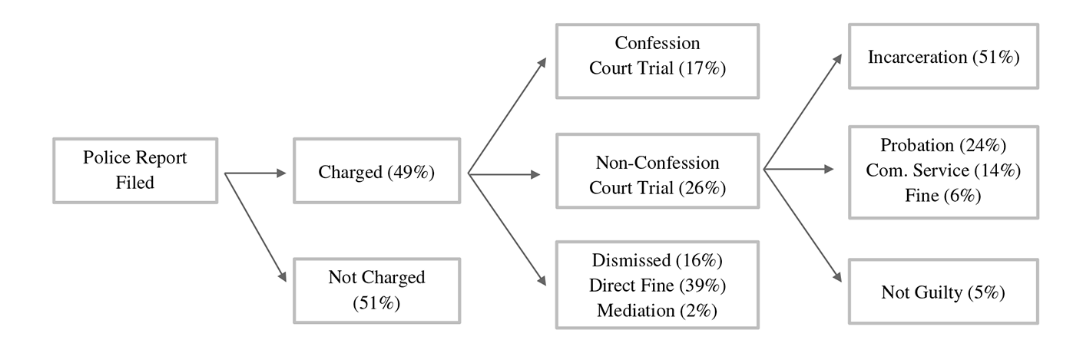
\includegraphics[scale=0.3]{../figures/Procedure.png}
  \end{center}
\item Norwegian law requires that judges be {\color{c2}randomly assigned} to cases (a few exceptions which are dropped)
\end{itemize}
}

\frame{
  \frametitle{Research Design}
  \begin{itemize}
  \item Model: \[ Y_{i,t} = \beta_{t}I_{i,0} + X_{i}'\theta_{t} + \eta_{i,t} \] 
  where $I_{i,0}$ indicates incarceration of person $i$ in period 0. \pause
  \item $X_{i}$ is a full set of court by year dummy variables.
  \item First stage:
   \[ I_{i,0} = \gamma {\color{c3}Z_{j(i)}} + X_{i}'\delta + \nu_{i,0} \]
   where $Z_{j(i)}$ is the {\color{c3}stringency} of judge $j$ assigned to person $i$:
   \[ Z_{j(i)} = \frac{\sum_{n\neq i} I_{n,0}\mathbf{1}\{j(n)=j\}}{\sum_{n\neq i}\mathbf{1}\{j(n)=j\}} \]
  \end{itemize}
}

\frame{
  \frametitle{Balance Test}
  \begin{center}
    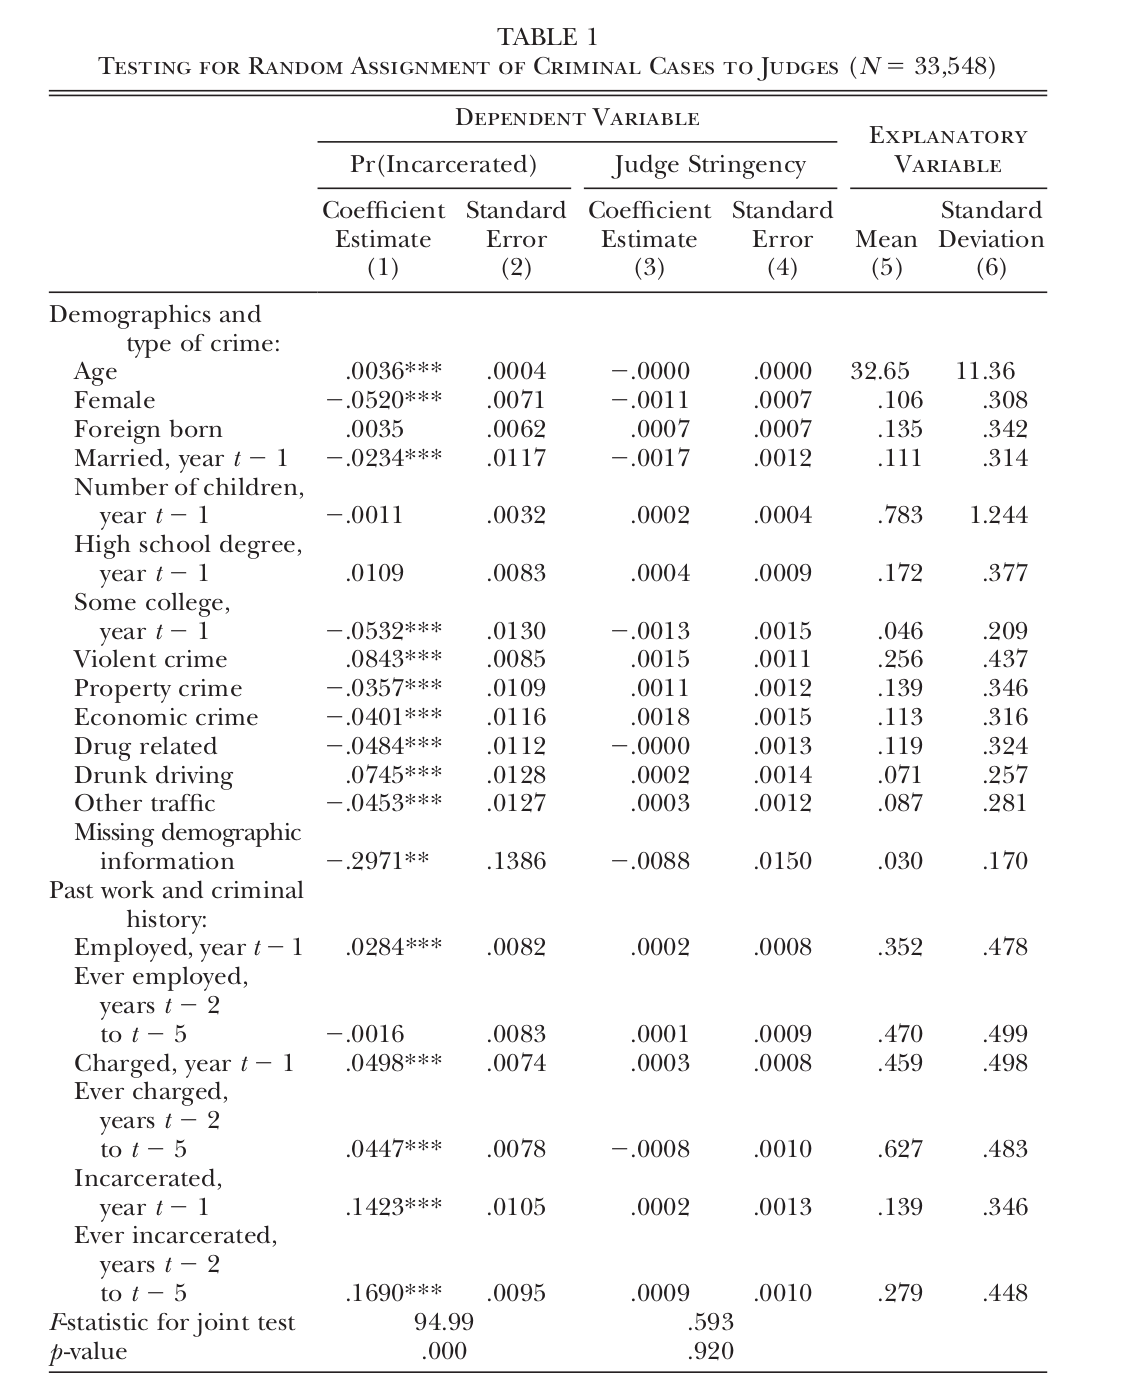
\includegraphics[scale=0.15]{../figures/BalanceTest.png}
  \end{center}
}

\frame{
  \frametitle{Instrument Strength}
  \begin{center}
    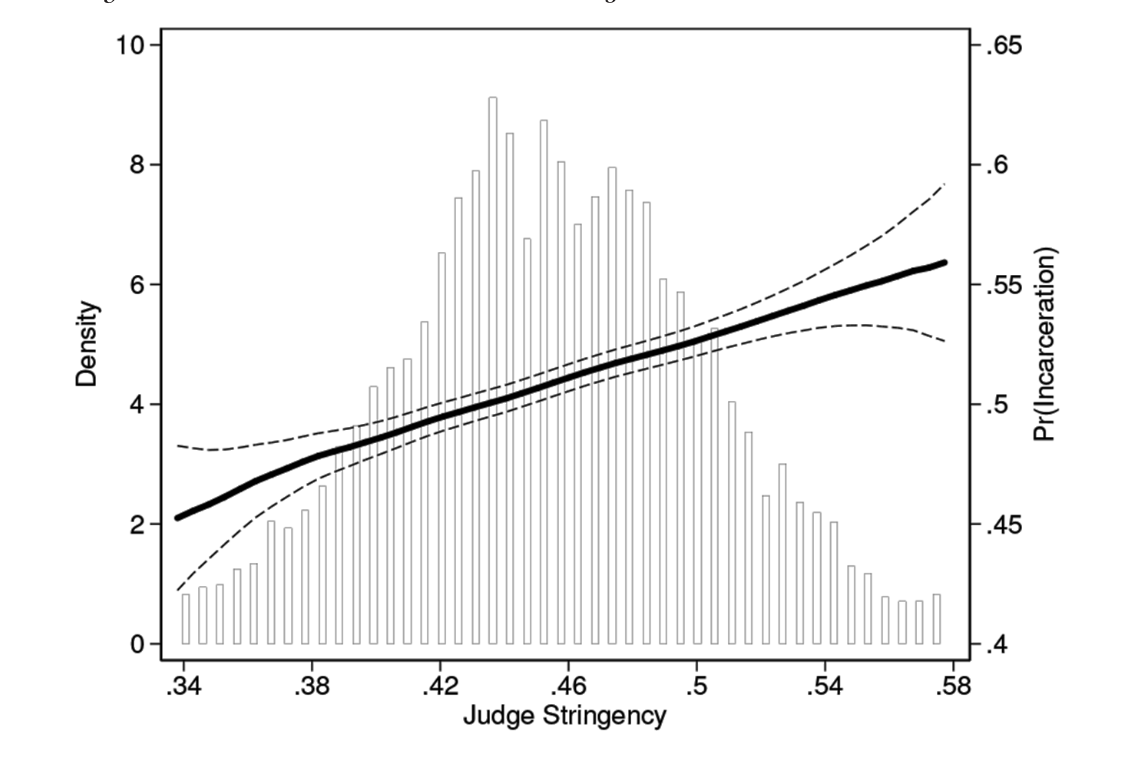
\includegraphics[scale=0.25]{../figures/IVStrength-1.png}
  \end{center}
}

\frame{
  \frametitle{Instrument Strength}
  \begin{center}
    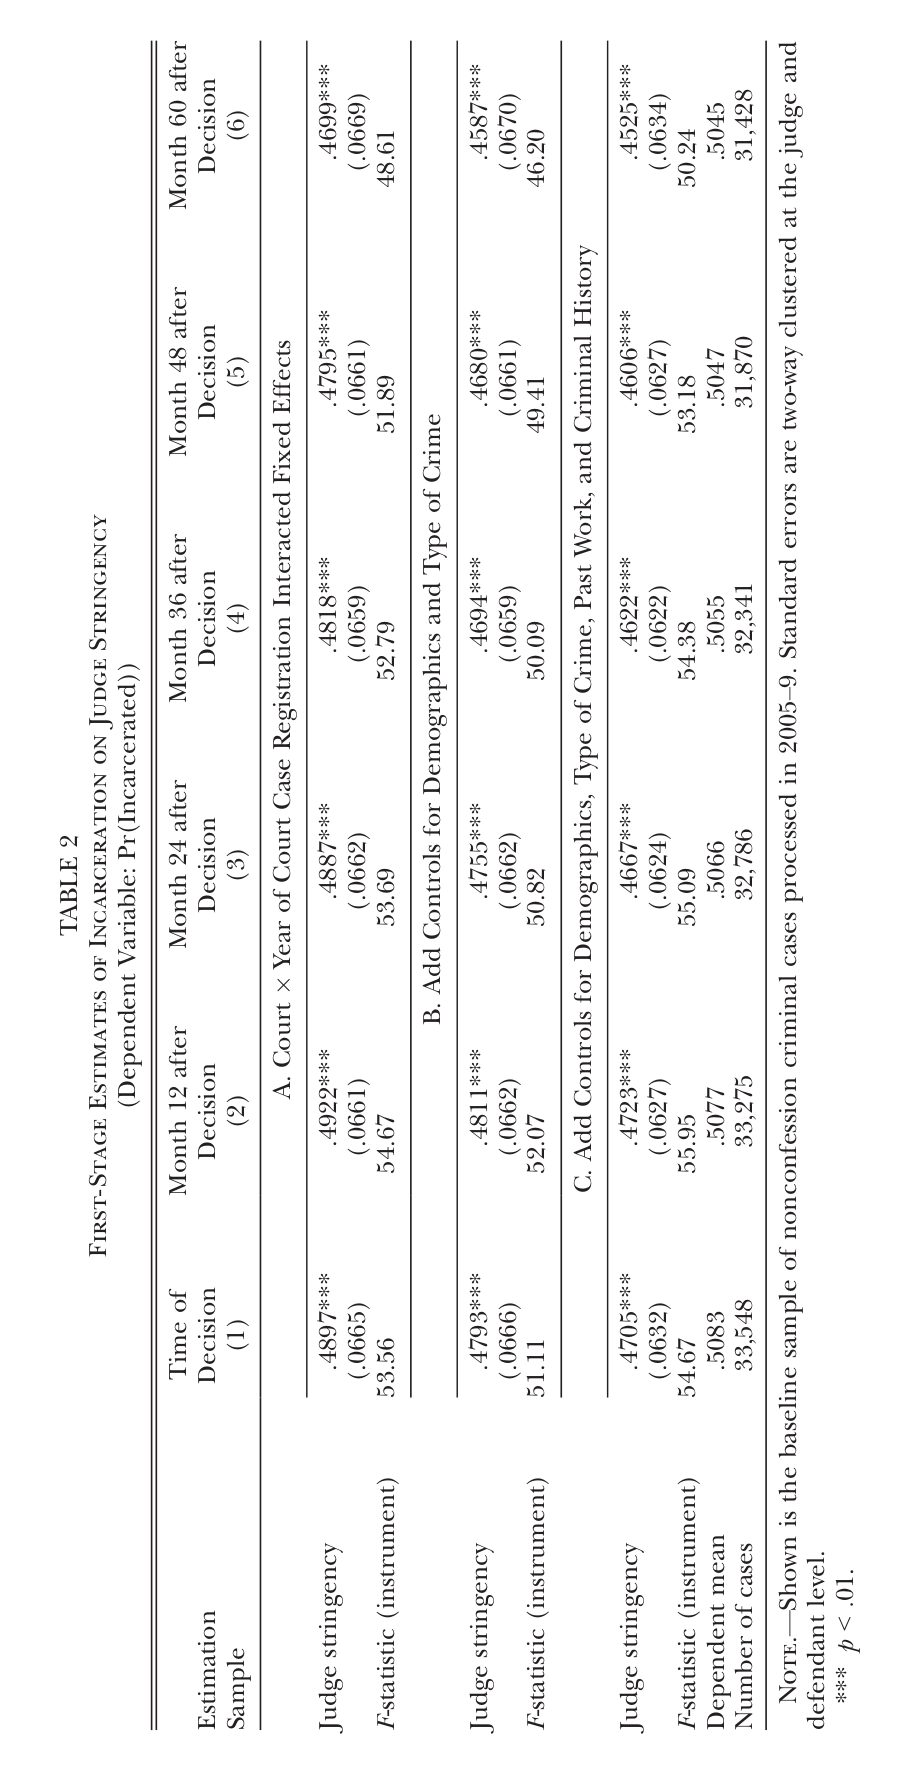
\includegraphics[scale=0.2,angle=270,origin=c]{../figures/IVStrength-2.png}
  \end{center}
}

\frame{
  \frametitle{An Aside on Instrument Monotonicity}
  \begin{itemize}
    \item If you read the paper you will find a lot of discussion on {\color{c2}instrument monotonicity}, which the paper tests for. \pause
    \item Monotonicity is only relevant if the treatment has {\color{c2}heterogeneous effects} (likely). \pause
    \item An instrument is monotonic if different values of the instrument either uniformly increase or decrease the probability of treatment for everyone. \pause
    \item Here this means that more strict judges would incarcerate all of the defendents that more lenient judges do.
    \item With a monotonic instrument, the TSLS estimand has a {\color{c2}Local Average Treatment Effect} interpretation, which you've seen before.
    \item You'll see more of this in recitation.
  \end{itemize}
}

\frame{
  \frametitle{Incarceration and Recidivism}
  \begin{center}
    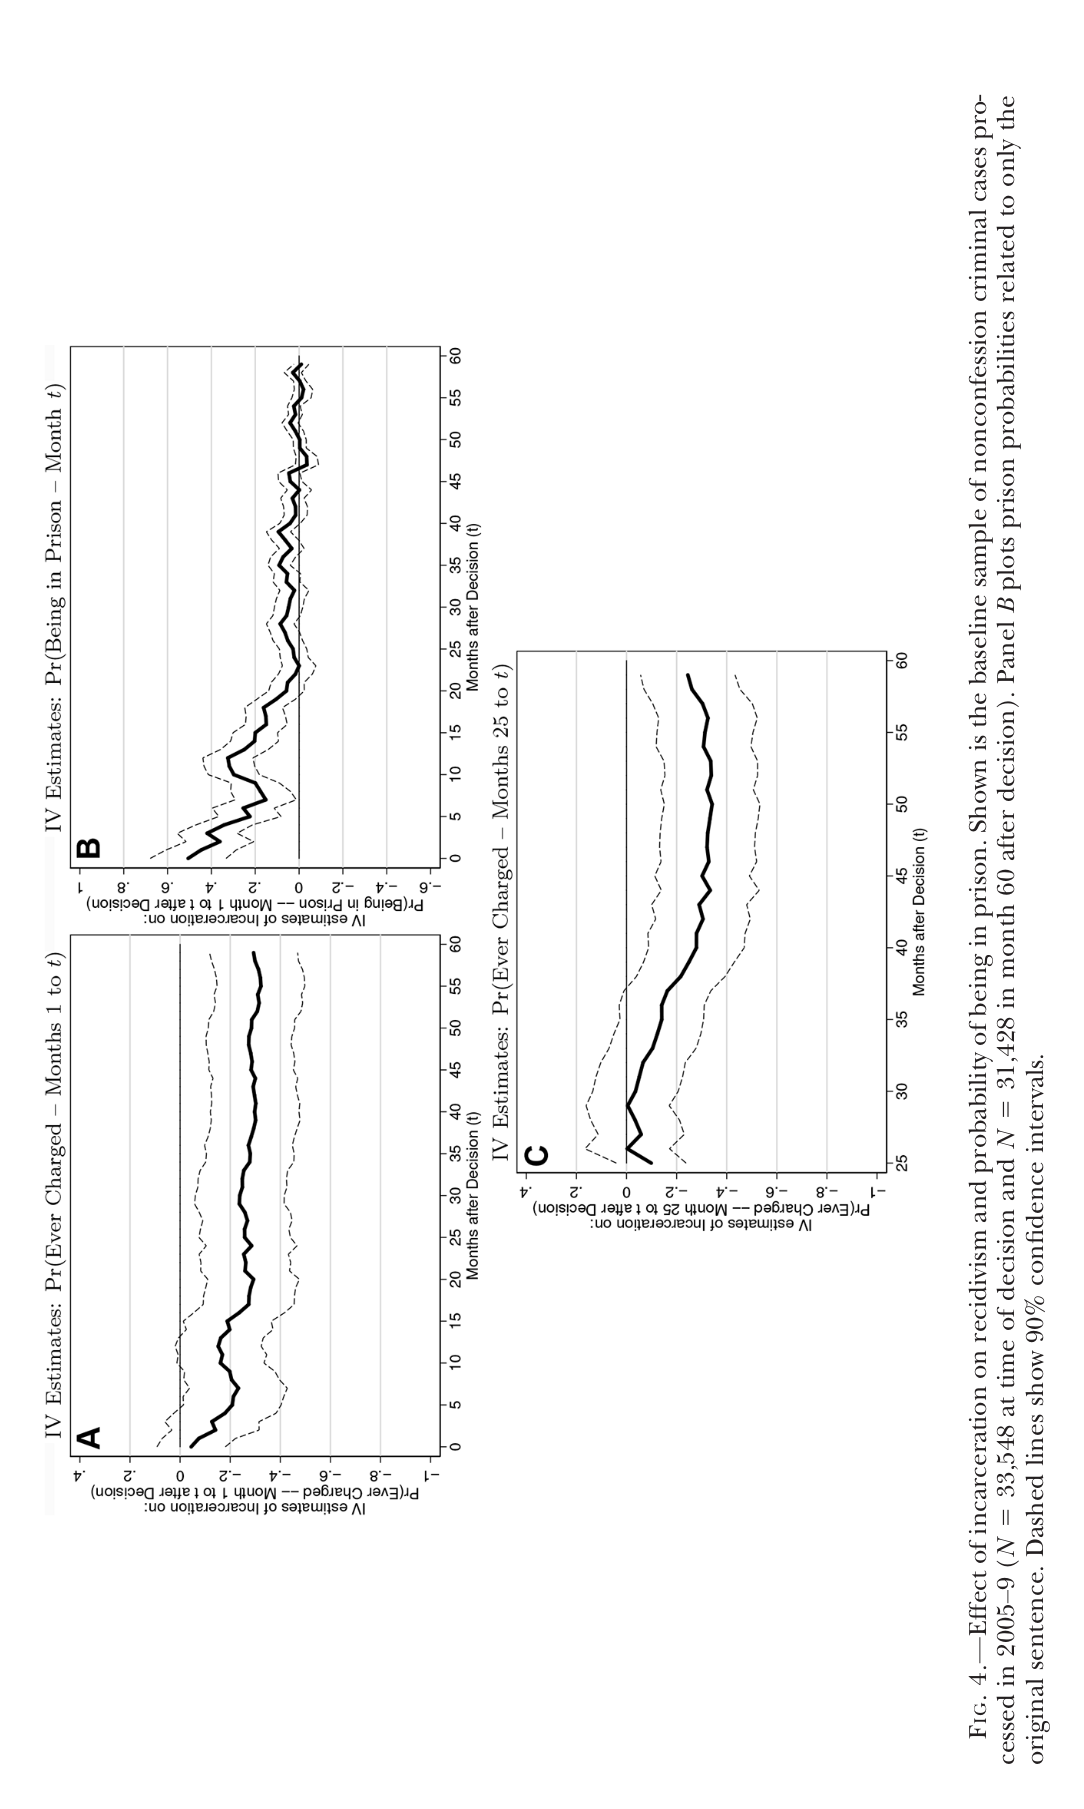
\includegraphics[scale=0.2,angle=270,origin=c]{../figures/Estimates-1.png}
  \end{center}
}

\frame{
  \frametitle{Incarceration and Recidivism}
  \begin{center}
    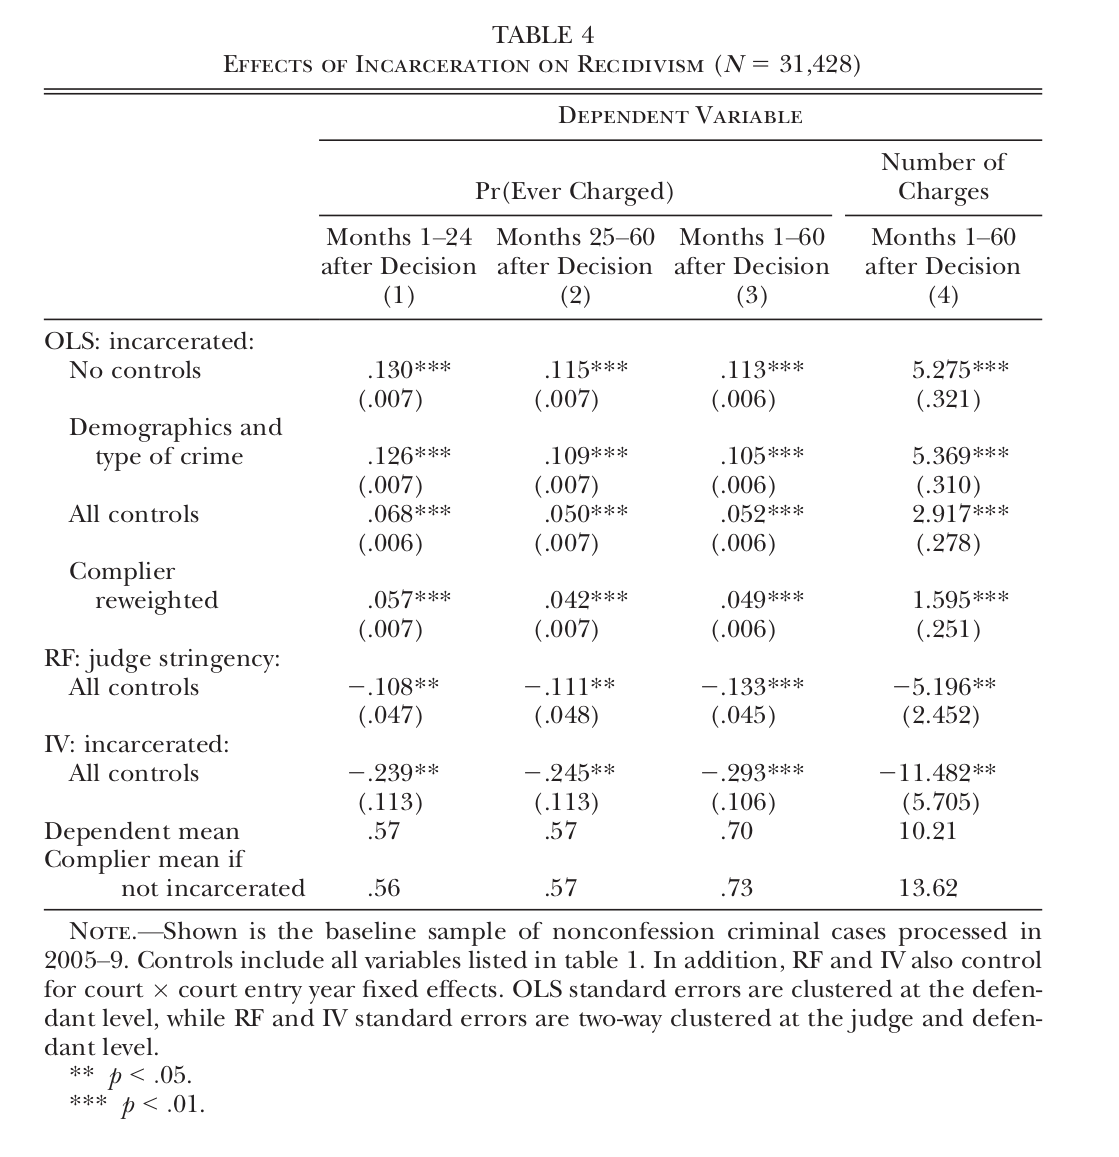
\includegraphics[scale=0.2]{../figures/Estimates-2.png}
  \end{center}
}

\frame{
  \frametitle{Incarceration and Recidivism}
  \begin{center}
    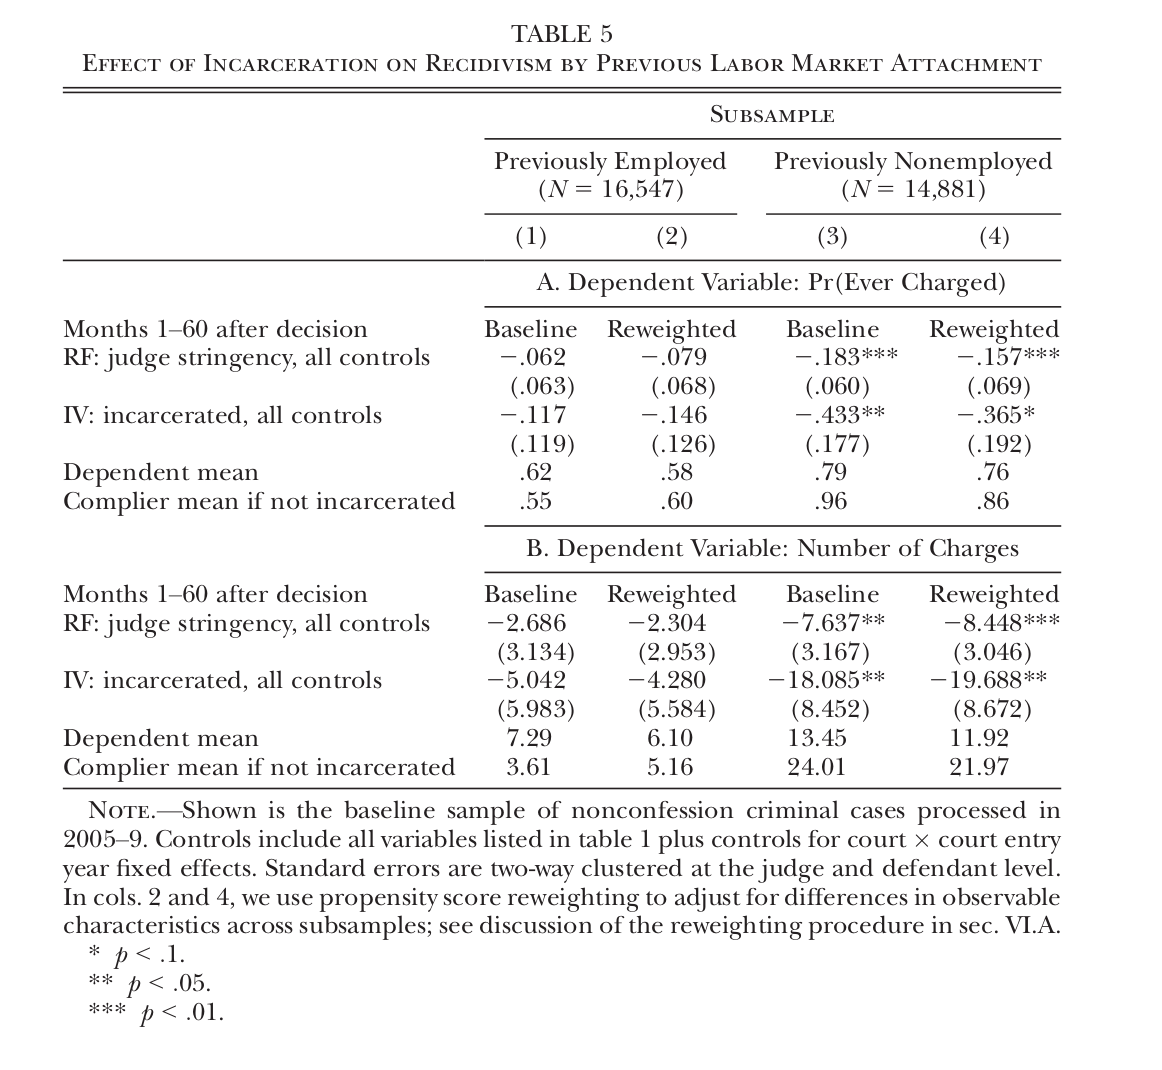
\includegraphics[scale=0.2]{../figures/Estimates-3.png}
  \end{center}
}

\frame{
  \frametitle{Incarceration and Recidivism}
  \begin{center}
    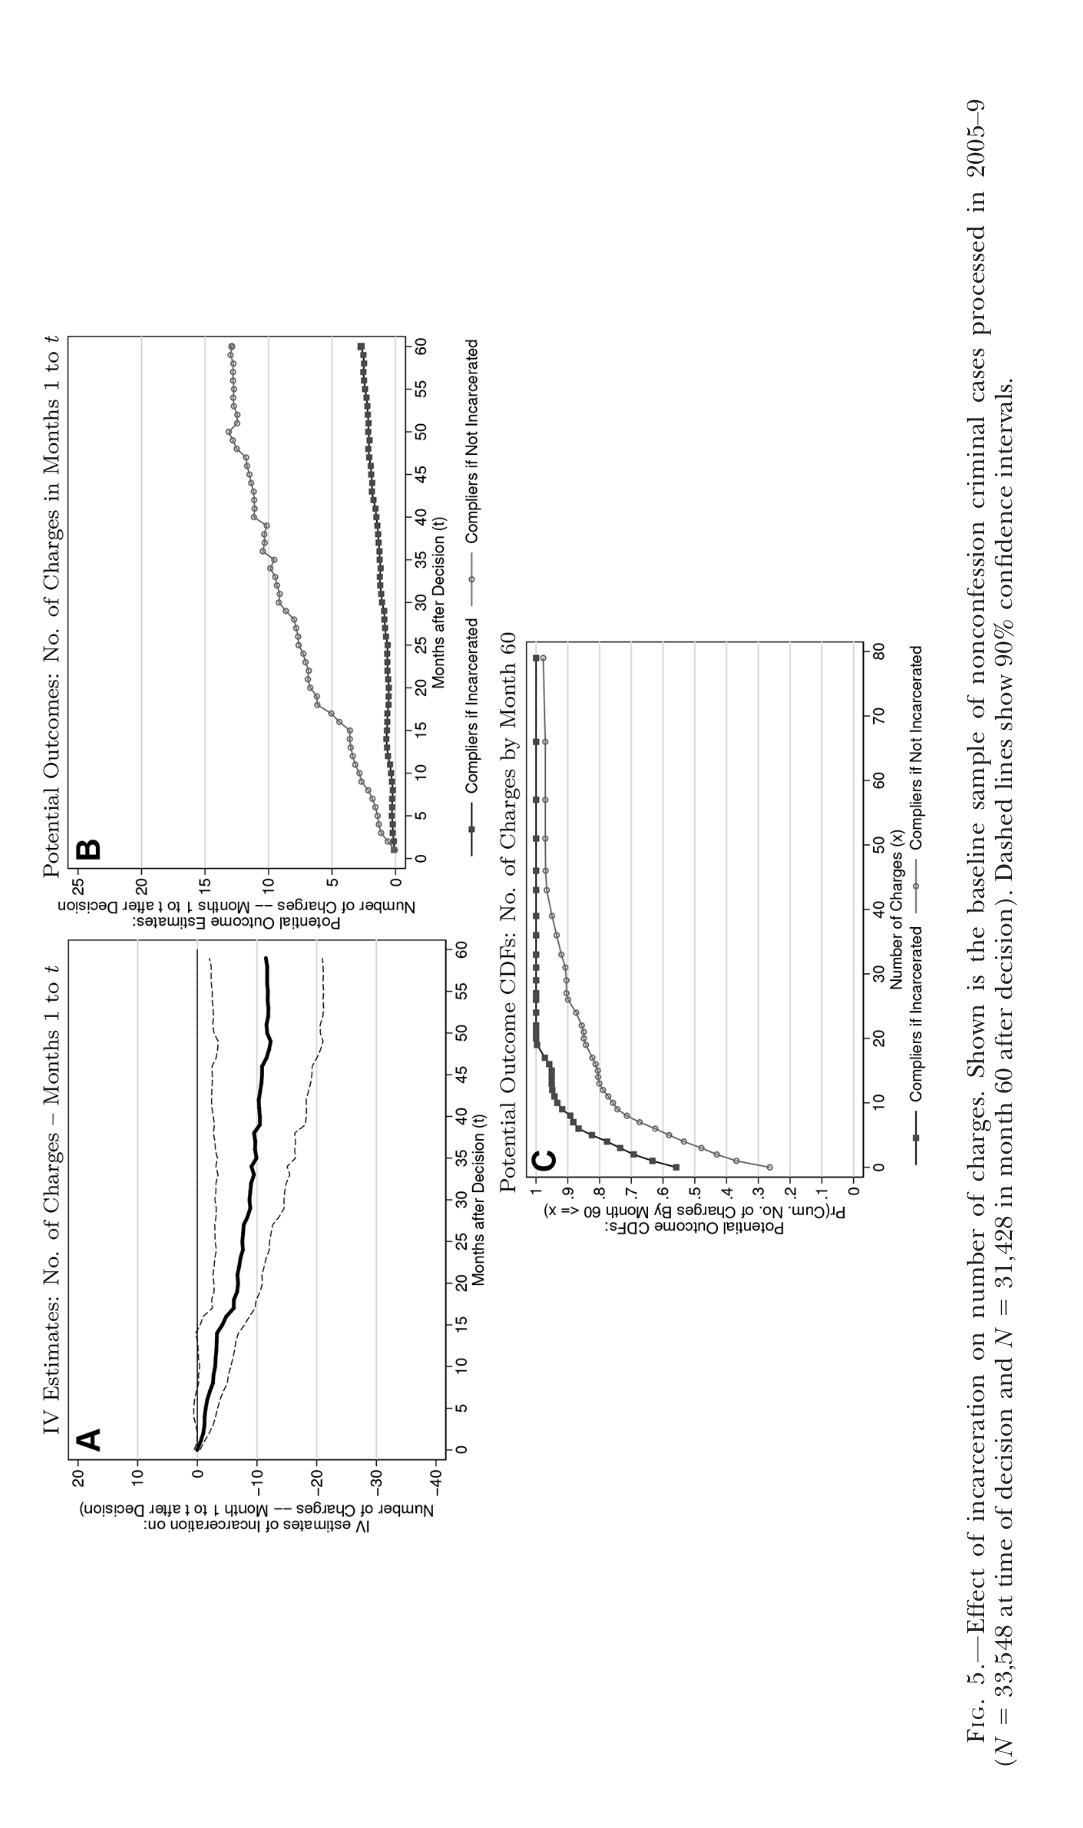
\includegraphics[scale=0.2,angle=270,origin=c]{../figures/Estimates3.png}
  \end{center}
}


\frame{
  \frametitle{Incarceration and Employment}
  \begin{center}
    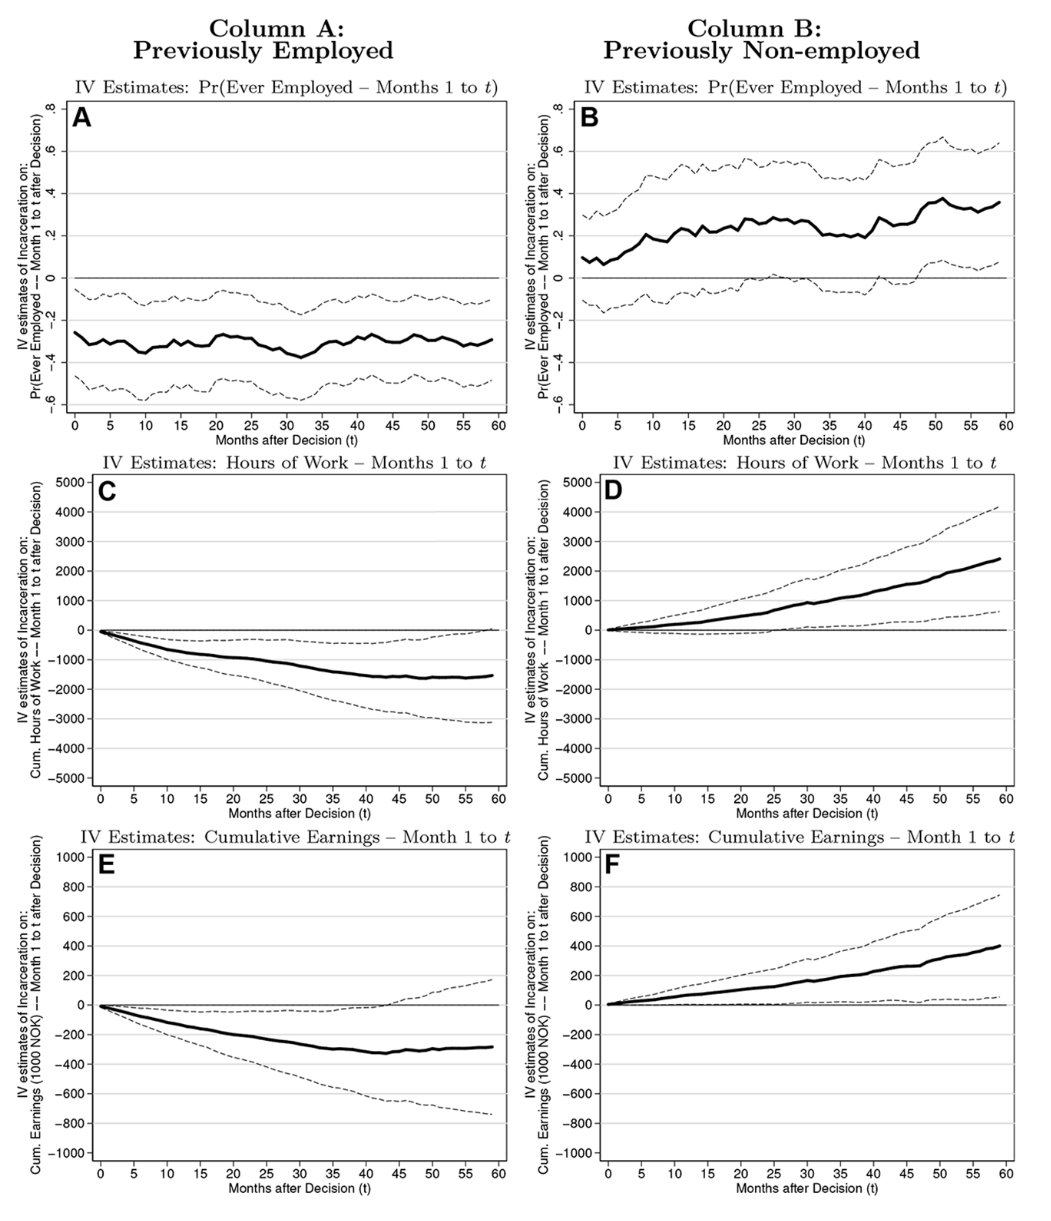
\includegraphics[scale=0.15]{../figures/Estimates-4.png}
  \end{center}
}

\frame{
  \frametitle{Other Exercises}
  The paper also:
  \begin{wideitemize}
    \item Tests for violations of instrument monotonicity \pause
    \item Tests for effects coming through other dimensions of judge decisions (fines, community service, etc). These would violate {\color{c2}instrument exclusion}. \pause
    \item Conducts a cost-benefit analysis (positive)
  \end{wideitemize}
}


\frame{
  \frametitle{Conclusion}
  \begin{itemize}
    \item The paper finds that incarceration reduces further criminal behavior and improves future employment outcomes.
    \item The effects are concentrated among those who were not working prior to incarceration.
    \item Some evidenc that the effect comes through the provision of job training programs in prison.
    \item Prison in Norway is {\color{c3}very different} from prison in the US.
  \end{itemize}

}


\end{document}

%%% Local Variables:
%%% mode: latex
%%% TeX-master: t
%%% End:
